\documentclass{beamer}
\title{The Impact of Anthropogenic Forcing on ENSO Amplitude}
\author{Ben Goldman}
\date{\today}
\usepackage{natbib}
\usepackage{tikz}
\usepackage{varwidth}
\usetikzlibrary{arrows,snakes,backgrounds}
\usetheme{metropolis}
\renewcommand{\bibsection}{}
\setbeamerfont{caption}{size=\tiny}

% \begin{frame}{Example Frame With Text and Image}
%   \begin{columns}
%     \column{0.5\textwidth}
%     \begin{itemize}
%     \item Here we go...
%     \end{itemize}
%     \column{0.5\textwidth}
%     \begin{figure}
%       \centering
%       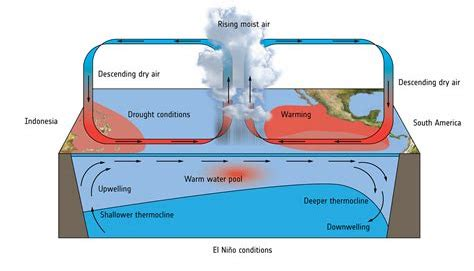
\includegraphics[width=\textwidth]{figures/example.jpg}
%       \caption{This is a very nice figure}
%       \label{fig:this}
%     \end{figure}
%   \end{columns}
% \end{frame}

\newcommand{\myfig}[3]{
  \begin{figure}
    \centering
    \includegraphics[width=\textwidth]{figures/#1}
    \caption{#2}
    \label{fig:#3}
  \end{figure}
}


\begin{document}

\maketitle

\section{Introduction}

\begin{frame}{Climate Change}

  \begin{columns}
    \column{0.6\textwidth}
    \begin{itemize}
    \item The earth is getting warmer. \citep{pachauri2014climate}
    \item Climate varies on different scales.
    \item Long-term trends and short-term noise.
    \item Forcing: any external factor that affects climate
      \begin{itemize}
      \item Greenhouse gasses
      \item Aerosols (natural: volcanic ash, artificial: smoke)
      \item Biomass burning
      \item Land use/cover (deforestation, desertification)
      \end{itemize}
    \end{itemize}
    \column{0.4\textwidth}
    \myfig{intro_fig_3.pdf}{Global mean land air temperature in GISSTEMP 4 dataset. \citep{gistemp2019giss} and \citep{lenssen2019improvements}}{this}
  \end{columns}
\end{frame}

\begin{frame}{El Niño}
  \begin{figure}
    \begin{columns}
      \column{0.5\textwidth}
      \begin{itemize}
      \item Warming and cooling of the Pacific Ocean.
      \item Affects human societies through temperature and rainfall. \citep{ropelewski1987global}
      \item May be affected by climate change.
      \end{itemize}
      \caption{Comparison of SST anomaly between 1975 La Niña event and 1997 El Niño event in HadISST 1 dataset. \citep{rayner2003global}}
      \column{0.5\textwidth}
      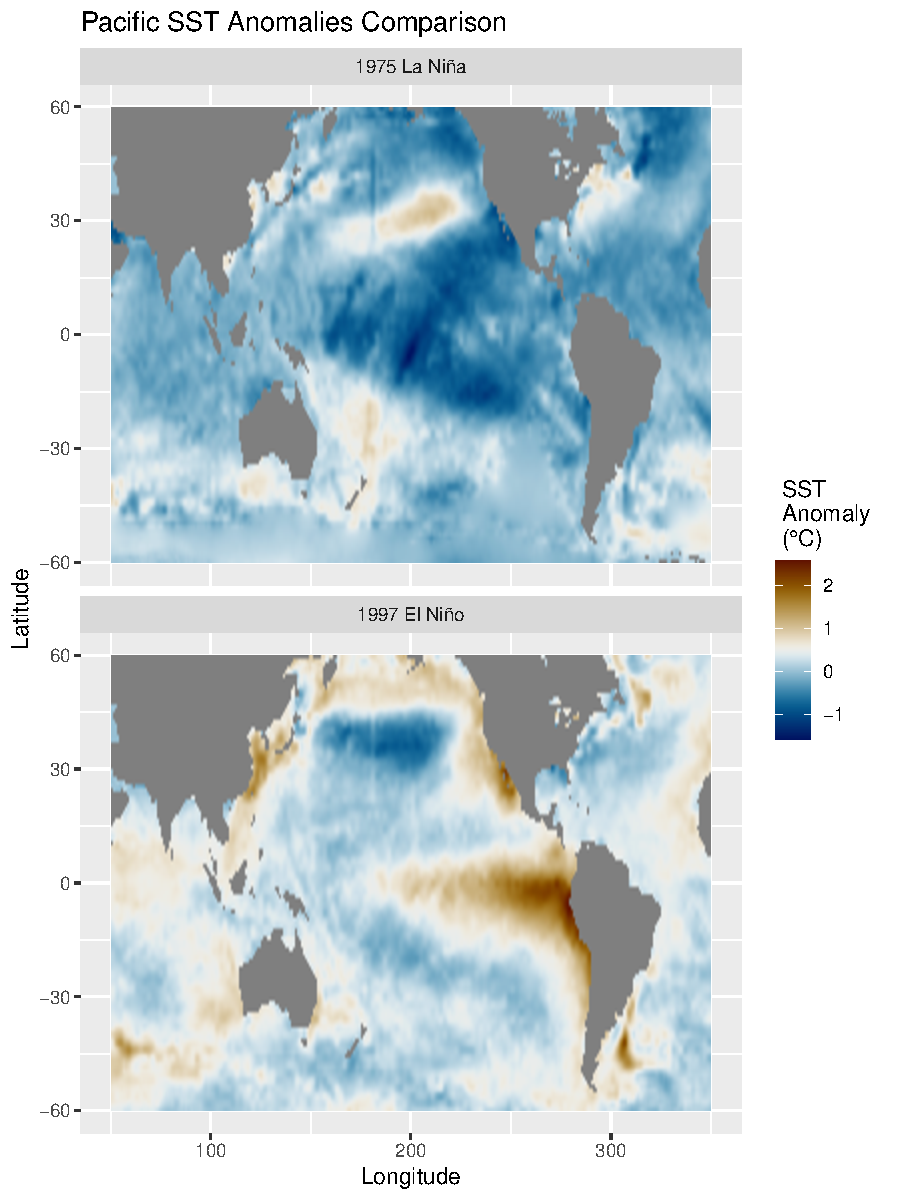
\includegraphics[width = \textwidth]{figures/intro_fig.pdf}
    \end{columns}
  \end{figure}
\end{frame}

\begin{frame}{Climate Simulation}

  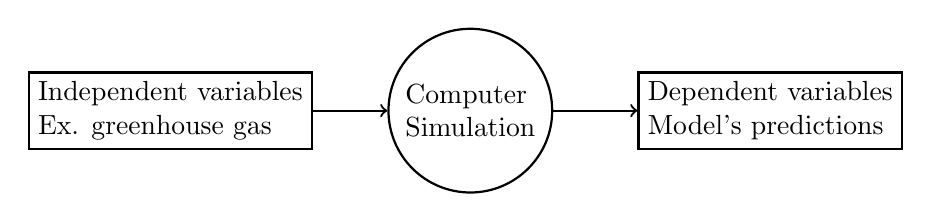
\begin{tikzpicture}[node distance = 1.5in, thick]

    \node (input) [rectangle, draw] {
      \begin{varwidth}{1.5in}
        Independent variables
        Ex. greenhouse gas
      \end{varwidth}};

    \node (model) [right of=input, circle, draw] {
      \begin{varwidth}{\linewidth}
        Computer\\Simulation
      \end{varwidth}};

    \node (output) [right of=model, rectangle, draw] {
      \begin{varwidth}{1.4in}
        Dependent variables
        Model's predictions
      \end{varwidth}};

    \draw [->] (input.east) -- (model.west);
    \draw [->] (model.east) -- (output.west);

  \end{tikzpicture}

\end{frame}

\begin{frame}{ENSO in the Future}
\end{frame}

\begin{frame}{Gap and Goal}

\end{frame}

\begin{frame}{Research Questions}

\end{frame}

\section{Data and Methods}

\begin{frame}{Ensembles: CESM1 and CESM2}

\end{frame}

\begin{frame}{Analysis Tools}
  \begin{columns}[t]
    \column{.33\textwidth}
    R:
    \begin{itemize}
    \item ncdf4
    \item zoo
    \item dplyr
    \item ggplot2
    \item WaveletComp
    \item reshape2
    \end{itemize}
    \column{.33\textwidth}
    Python:
    \begin{itemize}
    \item numpy
    \item pandas
    \item scipy
    \item matplotlib
    \item netCDF4
    \end{itemize}
    \column{.33\textwidth}
    Other:
    \begin{itemize}
    \item nco
    \end{itemize}
  \end{columns}

\end{frame}

\begin{frame}{Role of Mentor and Student}
  \begin{columns}[t]
    \column{.5\textwidth}
    Mentor:
    \begin{itemize}
    \item Suggest future methods
    \item Conduct parallel analysis to complement student work
    \item Provide raw precollected data
    \item Interpret data produced by student
    \item Review student writing
    \end{itemize}
    \column{.5\textwidth}
    Student:
    \begin{itemize}
    \item Analyze data on computer
    \item Produce graphics for analysis and publication
    \item Write documentation
    \item Suggest interpretations of data
    \end{itemize}
  \end{columns}

\end{frame}

\begin{frame}{Model Setup}
  Input:
  \begin{itemize}
  \item Observed forcing levels from 1850-2005
  \item Predicted forcing levels from 2005-2100
  \item \textbf{Simulation ran a total of 40 times with slightly different starting point}
  \item Control simulation with pre-1850 forcing levels
  \end{itemize}
  Model:
  \begin{itemize}
  \item CESM1 \citep{kay2015community}
  \item CESM2 \citep{danabasoglu2020community}
  \end{itemize}
  Output: Sea Surface Temperature (SST)
\end{frame}

\begin{frame}{Measuring ENSO Intensity}

  \tikzstyle{process}=[circle, draw=black!50,fill=black!20, line width = 0.2mm]
  \tikzstyle{data}=[rectangle, draw=blue!50,fill=blue!20, line width = 0.2mm]
  \begin{tikzpicture}[node distance = 1.5in, line width = 0.5mm]

    \node [data] (input) {
      \begin{varwidth}{1.5in}
        External forcing
      \end{varwidth}};

    \node [process] (model) [right of=input] {
      \begin{varwidth}{\linewidth}
        CESM1\\and\\CESM2
      \end{varwidth}};

    \node [data] (output) [right of=model] {
      \begin{varwidth}{1.2in}
        Sea surface temperature (SST)
      \end{varwidth}};

    \node [data] (nino) [below of=input] {
      \begin{varwidth}{1.4in}
        Niño 3.4 index
      \end{varwidth}};

    \node [process] (variance) [right of=nino] {
      \begin{varwidth}{1.4in}
        Windowed\\variance
      \end{varwidth}};

    \node [data] (intensity) [right of=variance] {
      \begin{varwidth}{1.4in}
        ENSO intensity
      \end{varwidth}};

    \draw [->] (input) to (model);
    \draw [->] (model) to (output);
    \draw [->] (output) to [out = 270, in = 90] (nino);
    \draw [->] (nino) to (variance);
    \draw [->] (variance) to (intensity);

  \end{tikzpicture}

\end{frame}

\begin{frame}{Signal and Noise}

\end{frame}

\begin{frame}{ENSO is Becoming Stronger}

\end{frame}

\begin{frame}{Single Forcing Ensembles}

\end{frame}

\begin{frame}{Influence of Aerosols and Greenhouse Gasses}

\end{frame}

\begin{frame}{Correlation With Ocean Temperature}

\end{frame}

\begin{frame}{Stratification}

\end{frame}

\section{Conclusion}

\begin{frame}{Conclusions}

\end{frame}

\begin{frame}{Discussion}

\end{frame}

\begin{frame}{Acknowledgments}

\end{frame}

\begin{frame}{References}
  \bibliographystyle{apalike}
  \fontsize{7pt}{7.2}\selectfont
  \bibliography{references.bib}
\end{frame}

\maketitle

\end{document}
